\subsection{Optimizations for Local Neighborhood-based Similarity search}
\label{sec:leiden}

Consider an undirected graph $G(V, E)$. For each vertex $u$ in the graph, we count the number of paths to each second order neighbor of $u$, i.e., we calculate $N(u) \cap N(w)$ for each $w \in N(N(u))$. We then use this to calculate two different neighbor similarity metrics, namely, Jaccard's coefficient (JC) and Hub-Promoted (HP) score \cite{gatadi2023lpcd}. By \textit{exploring only second order neighbors} of each vertex, we skip computing scores on pairs of vertices which have no neighbors in common, and thus have a similarity score of $0$. We parallelize this approach with OpenMP's \textit{dynamic} schedule, with a chunk size of $2048$, and optimize path counting and lookup with per-thread collision-free hashtables. Note that we only want to predict links between node pairs with top-$k$ similarity scores, with $k$ being a fraction of the number of edges in the original graph $|E|$. Accordingly, we use a per-thread min-heap based prediction list, which allows us to keep node pairs with top-$k$ scores (per thread), and evict the node pair with the lowest score once we have a node pair with a higher score. Once all vertices have been processed by the threads, we concatenate the prediction lists, sort them by similarity score in increasing order, and return only the top-$k$ links predicted. As an optimization, we convert the per-thread prediction lists into a min-heap only when the prediction lists is populated with $k$ entries. At this stage, predicting links on graph with $2.3$ million edges using $24$ threads takes $14$ seconds.

To further optimize link prediction, we note that low-degree nodes are users who have only a few connections in the social network. These users are more selective in accepting friend requests and are likely to form connections with people they have stronger, more meaningful relationships with, such as close friends and family. Thus, low-degree nodes confer significant similarity among their neighbors, while high-degree nodes generally do not (due to their lack of selectivity). Accordingly, for vertex $u$, we only explore neighbors of $v \in N(u)$ only if $degree(v) \leq D$ (where $D$ is the degree threshold for a neighbor of $u$). With $D = 4$, predicting links on the $2.3$ million edge graph\ignore{ using $24$ threads} now takes only $10$ milliseconds. Figure \ref{fig:about-pruning} shows an explanation of this approach. Here, vertex $4$ is considered for similarity score calculation with vertex $1$, as they are both linked to a common low-degree neighbor, i.e., vertex $2$. However, neighbors of high-degree vertex $3$ are not considered for score calculation.


TODO.

% \input{src/fig-leidenopt-runtime}
% \input{src/fig-leidenopt-modularity}
% \input{src/fig-leiden-pass}




\subsection{Our optimized Leiden implementation}

We now explain the implementation of TODO.


\subsubsection{Main step of GVE-Leiden}

TODO.

% \begin{algorithm}[hbtp]
\caption{GVE-Leiden: Our parallel Leiden algorithm.}
\label{alg:leiden}
\begin{algorithmic}[1]
\Require{$G$: Input graph}
\Require{$C$: Community membership of each vertex}
\Require{$G'$: Input/super-vertex graph}
\Require{$C'$: Community membership of each vertex in $G'$}
\Require{$K'$: Total edge weight of each vertex}
\Require{$\Sigma'$: Total edge weight of each community}
\Ensure{$G'_{C'}$: Community vertices (CSR)}
\Ensure{$H_t$: Collision-free per-thread hashtable}
\Ensure{$l_i$, $l_j$: Number of iterations performed (per pass)}
\Ensure{$l_p$: Number of passes performed}
\Ensure{$\tau$: Per iteration tolerance}
\Ensure{$\tau_{agg}$: Aggregation tolerance}

\Statex

\Function{leiden}{$G$} \label{alg:leiden--begin}
  \State Vertex membership: $C \gets [0 .. |V|)$ \textbf{;} $G' \gets G$ \label{alg:leiden--initialization}
  \ForAll{$l_p \in [0 .. \text{\small{MAX\_PASSES}})$} \label{alg:leiden--passes-begin}
    \State $\Sigma' \gets K' \gets vertexWeights(G')$ \textbf{;} $C' \gets [0 .. |V'|)$ \label{alg:leiden--reset-weights}
    \State $l_i \gets leidenMove(G', C', K', \Sigma', \tau)$ \label{alg:leiden--local-move}
    \State $C'_B \gets C'$ \textbf{;} $C' \gets [0 .. |V'|)$ \textbf{;} $\Sigma' \gets K'$ \label{alg:leiden--reset-again}
    \State $l_j \gets leidenRefine(G', C'_B, C', K', \Sigma', \tau)$ \label{alg:leiden--refine}
    \If{$l_i + l_j \le 1$} \textbf{break} \Comment{Globally converged?} \label{alg:leiden--globally-converged}
    \EndIf
    \State $|\Gamma|, |\Gamma_{old}| \gets$ Number of communities in $C$, $C'$
    \If{$|\Gamma|/|\Gamma_{old}| > \tau_{agg}$} \textbf{break} \Comment{Low shrink?} \label{alg:leiden--aggregation-tolerance}
    \EndIf
    \State $C' \gets$ Renumber communities in $C'$ \label{alg:leiden--renumber}
    \State $C \gets$ Lookup dendrogram using $C$ to $C'$ \label{alg:leiden--lookup}
    \State $G' \gets leidenAggregate(G', C')$ \label{alg:leiden--aggregate}
    \State $\tau \gets \tau / \text{\small{TOLERANCE\_DROP}}$ \Comment{Threshold scaling} \label{alg:leiden--threshold-scaling}
  \EndFor \label{alg:leiden--passes-end}
  \State $C \gets$ Lookup dendrogram using $C$ to $C'$ \label{alg:leiden--lookup-last}
  \Return{$C$} \label{alg:leiden--return}
\EndFunction \label{alg:leiden--end}
\end{algorithmic}
\end{algorithm}

% \input{src/alg-leidenlm}
% \input{src/alg-leidenre}
% \input{src/alg-leidenag}
\begin{figure*}[hbtp]
  \centering
  \subfigure[Standard approach]{
    \label{fig:about-pruning--01}
    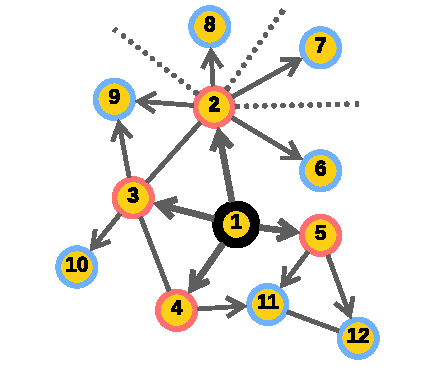
\includegraphics[width=0.31\linewidth]{out/about-pruning-01.pdf}
  }
  \subfigure[Disregard hubs with degree $> 8$]{
    \label{fig:about-pruning--02}
    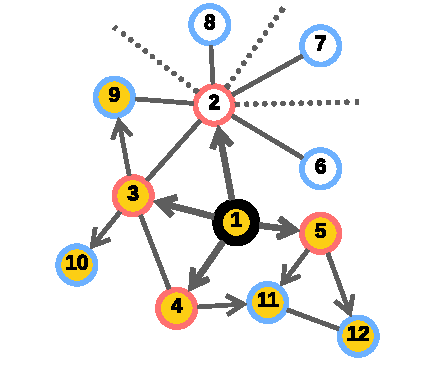
\includegraphics[width=0.31\linewidth]{out/about-pruning-02.pdf}
  }
  \subfigure[Disregard hubs with degree $> 4$]{
    \label{fig:about-pruning--03}
    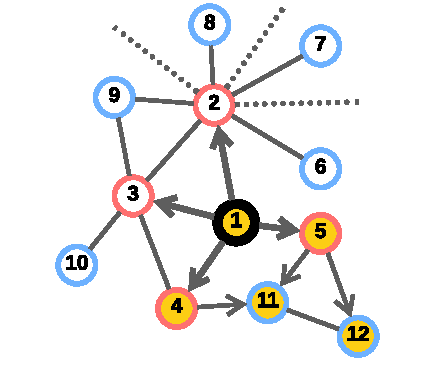
\includegraphics[width=0.31\linewidth]{out/about-pruning-03.pdf}
  } \\[-2ex]
  \caption{Illustration of our neighborhood-based link prediction approach, which disregards large hubs (first-order neighbors with high degree). The approach applies to each vertex in the graph. Here, we focus on the neighborhood of a vertex $1$ in the graph. The current vertex $1$ is outlined in black, its first-order neighbors in red, and its second-order neighbors in blue. Edge directions indicate traversal, with some second order vertices omitted for simplicity (dotted edges). (a) Depicts the standard approach, which considers all second-order neighbors of vertex $1$. (b) Presents our approach, which considers only second-order neighbors linked to $1$ through a small hub (degree $\leq 8$). This pruning reduces runtime and enhances prediction quality. (c) Illustrates our approach, where vertices with degree $> 4$ are considered large hubs.}
  \label{fig:about-pruning}
\end{figure*}

\begin{figure*}[hbtp]
  \centering
  \subfigure[Relative runtime (logarithmic scale), of each link prediction method]{
    \label{fig:adjust-mindegree--runtime}
    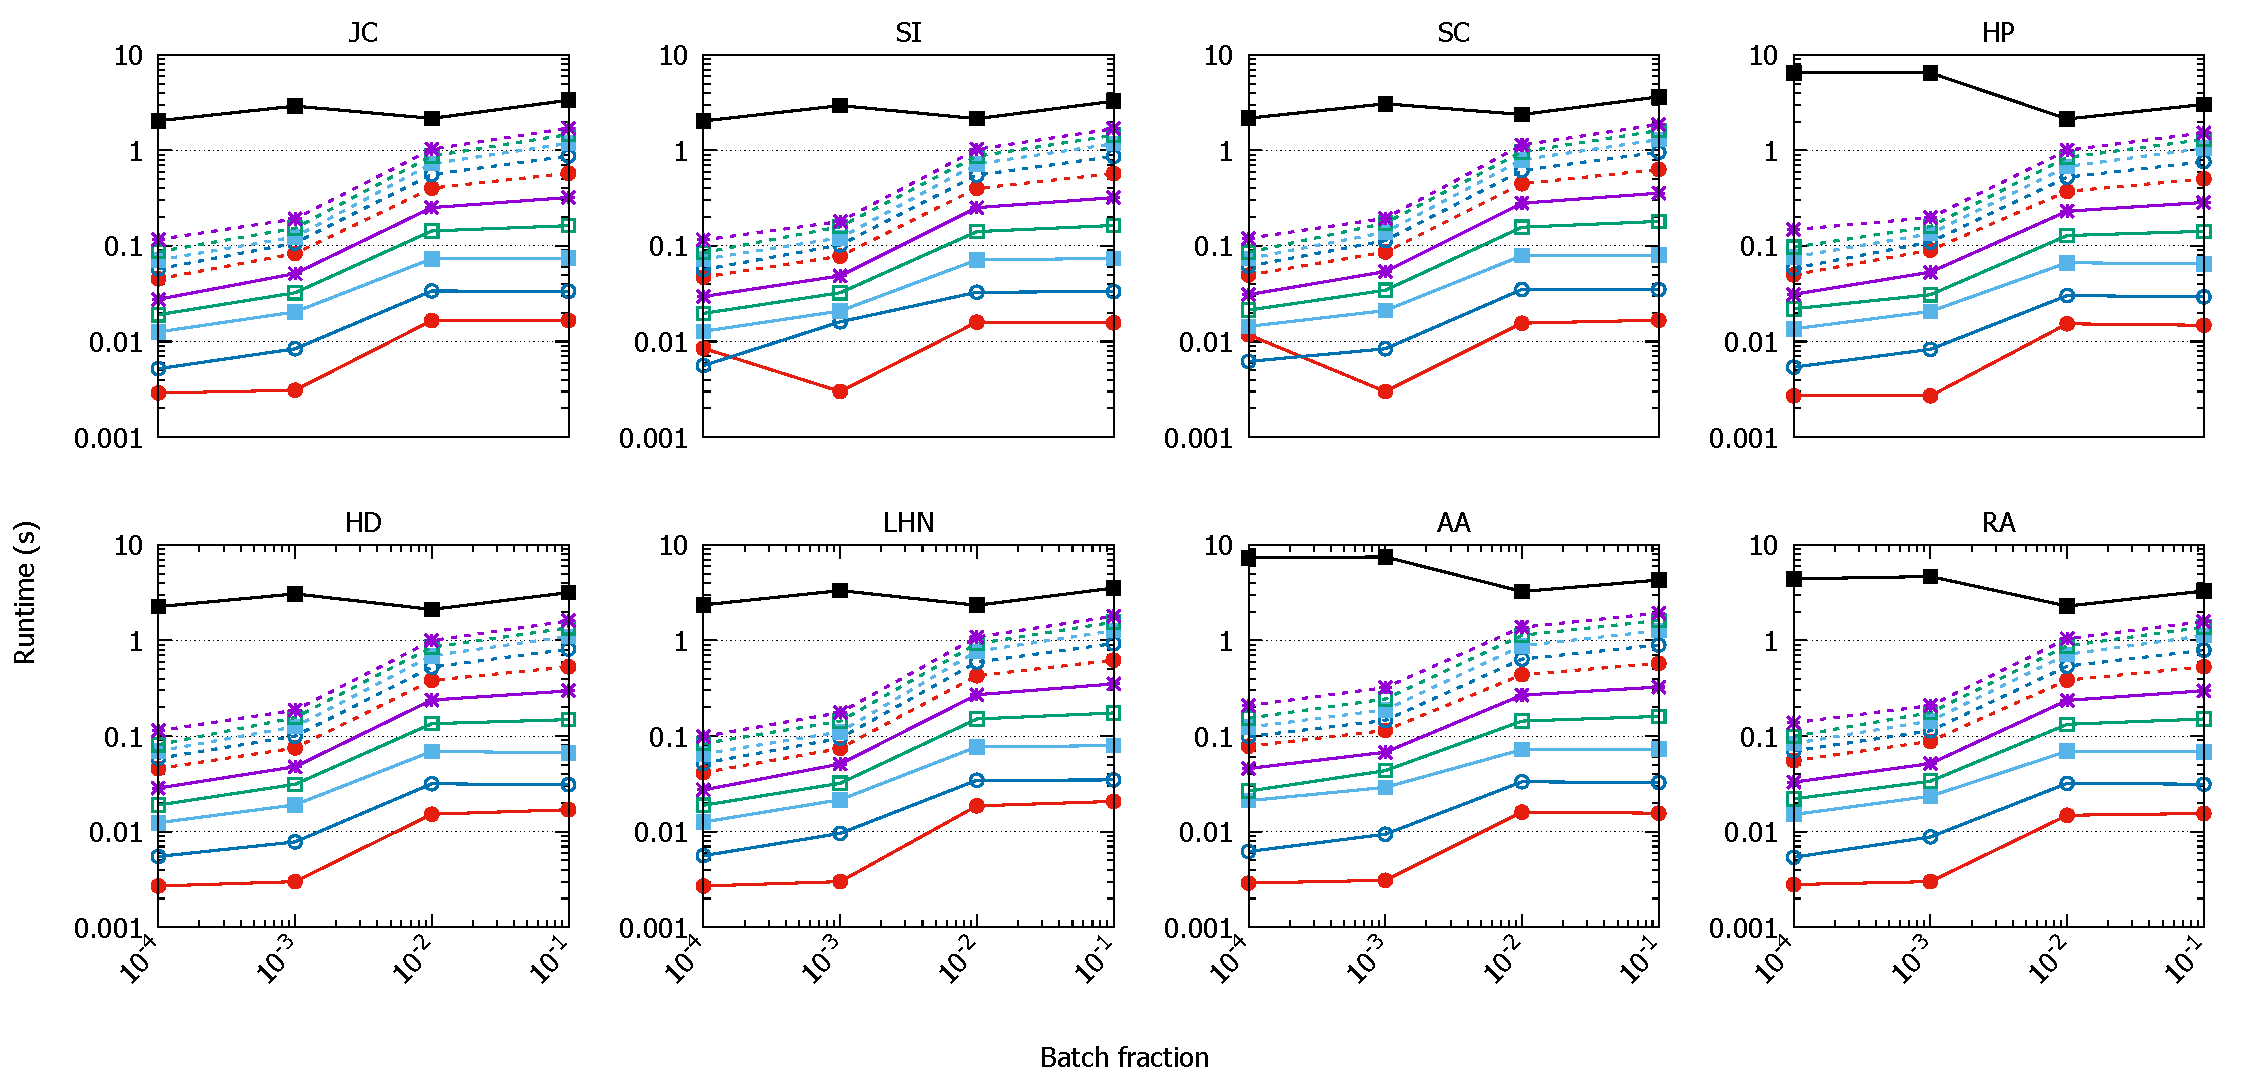
\includegraphics[width=0.98\linewidth]{out/adjust-mindegree-runtime.pdf}
  }
  \subfigure[F1 score of predicted links (logarithmic scale), of each link prediction method]{
    \label{fig:adjust-mindegree--precision}
    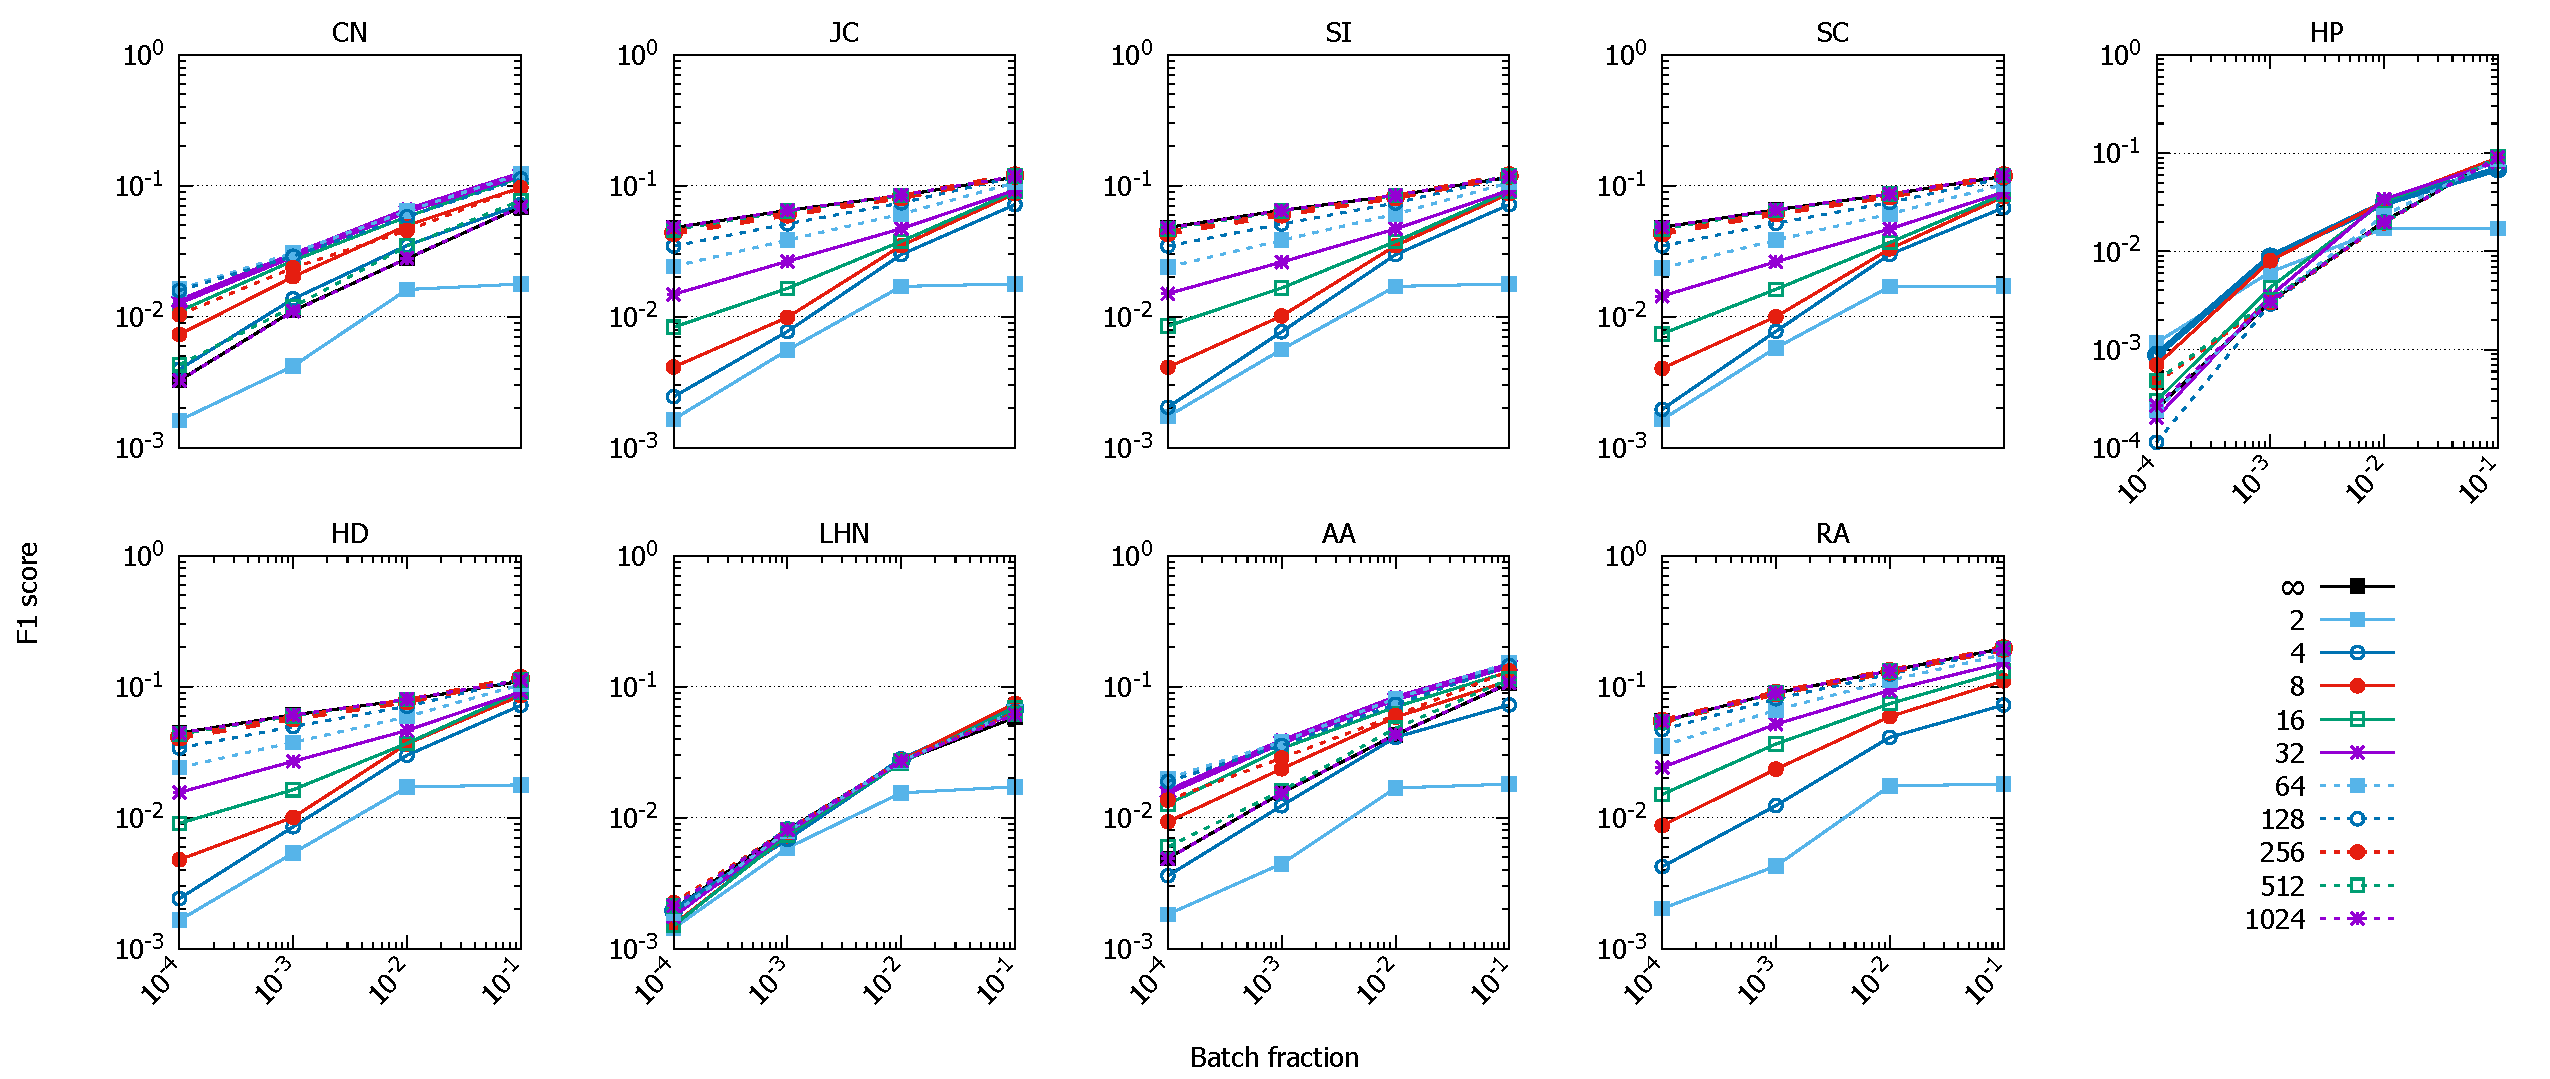
\includegraphics[width=0.98\linewidth]{out/adjust-mindegree-f1score.pdf}
  } \\[0ex]
  \caption{Impact of adjusting the \textit{MAX\_MEDIATOR\_DEGREE} from $2$ to $1024$ (in multiples of $2$), and to $\infty$, on the runtime (in seconds, log-scale), and precision of predicted links (in percentage, log scale), of each neighbor-based link prediction method, on batch sizes of $10^{-4}|E|$ to $0.1|E|$. The full form of each link prediction method is given in Section X.}
  \label{fig:adjust-mindegree}
\end{figure*}



\subsubsection{Local-moving phase of GVE-Leiden}

TODO.


\subsubsection{Refinement phase of GVE-Leiden}

TODO.


\subsubsection{Aggregation phase of GVE-Leiden}

TODO.




\subsection{Finding disconnected communities}

TODO.
